\begin{chapter}{Experimentos} \label{cap:experimentos}

Com o intuito de analisar os algoritmos da seção anterior, especialmente tempos de execução e médias das quantidades de reversões para obter uma solução, criamos testes utilizando dados simulados, divididos em três categorias. A primeira categoria usa como entrada permutações aleatórias (PR), permutações do tipo identidade embaralhadas uma única vez. Nestes testes, nosso esforço está voltado em observar o tempo de execução e a quantidade média de reversões necessárias para ordenar a instância do problema. A segunda categoria dos testes é utilizando permutações geradas a partir de reversões aleatórias (PGR), que são permutações também construídas a partir da permutação identidade, porém com múltiplos embaralhamentos, sendo nosso foco observar o comportamento dos resultados dos algoritmos em função da quantidade de embaralhamentos. Por fim, a terceira categoria de testes é composta por permutações de Gollan (PG) que, por suas propriedades especiais, necessitam de mais iterações dos algoritmos, sendo o foco da análise do tempo de execução em função do tamanho da permutação. Para maior precisão de nossas análises, os dados utilizados nos experimentos foram construídos a partir da média dos resultados de vários testes, com o intuito de diminuir ruídos na apresentação dos resultados. 
    
Os experimentos foram realizados em uma máquina com as seguintes especificações: processador Intel Dual Core 3,5 Ghz, 8 Gb de memória, sistema operacional Manjaro Linux e linguagem de programação Python3. 

\section{Experimentos com algoritmo \textit{Branch and Bound}}

\subsection{Permutações de Gollan}

No primeiro de nossos experimentos geramos PGs com tamanhos de 6 até 14 elementos, mantendo esse intervalo com o intuito de não ultrapassar o limite de 30 minutos estipulado para resolução de cada permutação. Especificamente neste conjunto de testes optamos por não executar múltiplas instâncias, ou seja, gerar várias PGs e calcular uma média dos resultados, por alguns motivos: o desempenho do algoritmo BnB não é bom e pelo fato do esforço computacional necessário para se ordenar uma permutação de Gollan ser alto. Note que na figura \ref{Grafico1}, a curva se mantém modesta inicialmente e a partir de um determinado ponto (tamanho da permutação $\ge 14$) apresenta uma explosão, crescendo rapidamente. Por este comportamento visto no gráfico podemos pressupor que estendendo esse gráfico para PGs com mais elementos, essa curva se assemelharia cada vez mais a de uma função exponencial, que é condizente com a complexidade do algoritmo BnB.

\begin{figure}[H]
\centering
  \begin{minipage}[b]{0.5\textwidth}
    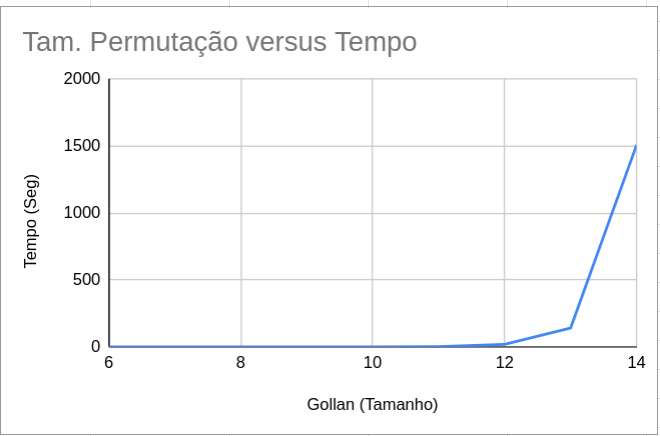
\includegraphics[width=\textwidth]{Imagens/Analises/B_PG2.png}
    \caption{\label{Grafico1}Gráfico da curva das PGs usando \textit{Branch and Bound}.}
  \end{minipage}
\end{figure}
    
\subsection{Permutações aleatórias}

A figura \ref{Grafico2} apresenta o gráfico de nossas análises utilizando PRs como entrada do algoritmo exato. Os resultados obtidos foram calculados a partir da média de 20 instâncias de teste e o intervalo do número de elementos das permutações foi de 9 elementos até 21 elementos. A partir de 21 elementos o tempo de execução dos testes ultrapassaria um limite de 6,5 horas que estipulamos e, por isso, não prosseguimos com testes maiores. A curva do gráfico esboça o comportamento do algoritmo exato e, assim como no experimento anterior, podemos inferir que estendendo este gráfico, seu tempo de execução se comportaria como uma função exponencial no tamanho da entrada.

\begin{figure}[H]
  \centering
  \begin{minipage}[b]{0.5\textwidth}
    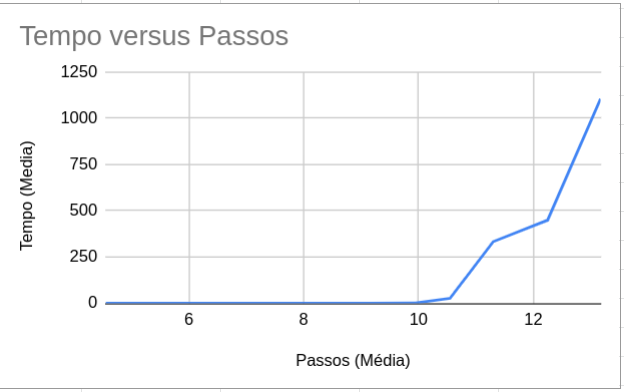
\includegraphics[width=\textwidth]{Imagens/Analises/B_PR2.png}
    \caption{\label{Grafico2}Gráfico da curva das análises usando PR como entrada para o algoritmo BnB.}
  \end{minipage}
\end{figure}

\subsection{Permutações geradas por reversões aleatórias}

A figura \ref{Grafico3} apresenta o gráfico de nossas análises referentes a PGRs como entrada do algoritmo BnB utilizando permutações de tamanho fixo de 30 elementos que são embaralhadas aplicando de 4 a 16 reversões, com incrementos de 1 em 1 para cada instância. Os resultados foram obtidos a partir de uma média de 20 testes. Podemos visualizar que ao longo do crescimento da quantidade de reversões de embaralhamento, a média da quantidade de reversões para ordenação também se mantém crescente, mas começa a se distanciar da curva de embaralhamento. Nossas estimativas são que, se pudéssemos estender estes testes, esse distanciamento seria mais evidente. Optamos pelo limite de 16 reversões, já que para prosseguir com um número maior gastaríamos um tempo superior a 5,5 horas, que foi nosso teto estipulado para cada conjunto destas análises.

\begin{figure}[H]
  \centering
  \begin{minipage}[b]{0.5\textwidth}
    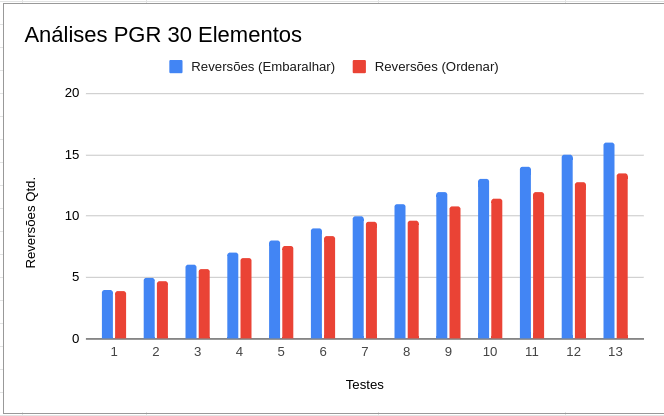
\includegraphics[width=\textwidth]{Imagens/Analises/B_PGR3.png}
    \caption{\label{Grafico3}Gráfico  de barras comparativas entre reversões usando o algoritmo \textit{Branch and bound}.}
  \end{minipage}
\end{figure}

\section{Experimentos com algoritmo \textit{Greedy}}

\subsection{Permutações de Gollan}

A figura \ref{Grafico4}, apresenta o gráfico de nossos experimentos utilizando PGs como entrada para o algoritmo \textit{Greedy}, com a quantidade de elementos da PG em um intervalo entre 10 e 495 elementos, com uma variação de 5 elementos incrementados a cada conjunto de testes, com os resultados obtidos a partir de uma média de 100 testes. É interessante observar que na curva de crescimento do tempo, um pico é apresentado a cada 10 elementos, comportamento este que podemos atribuir ao fato das PGs serem um tipo especial de permutação. 

\begin{figure}[H]
  \centering
  \begin{minipage}[t]{0.5\textwidth}
    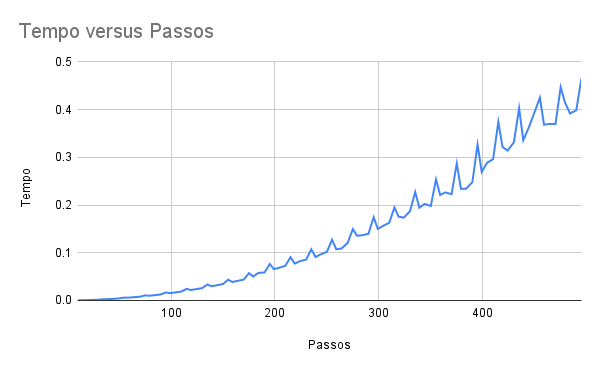
\includegraphics[width=\textwidth]{Imagens/Analises/G_PG2.png}
    \caption{\label{Grafico4} Gráfico da curva de PG como entrada do algoritmo \textit{Greedy}.}
  \end{minipage}
\end{figure}
    
\subsection{Permutações aleatórias}
    
A próxima análise representada na figura \ref{Grafico5} é referente aos experimentos utilizando PRs como entrada do algoritmo. Este conjunto de testes gerou as permutações mais extensas, demonstrando crescimento contínuo do tempo de execução, mas com alguns picos na média do tempo de execução em relação à média de passos de ordenação. As análises foram feitas utilizando permutações em um intervalo de 250 a 7750 elementos, com uma variação de 250 elementos incrementados a cada teste, com os resultados obtidos a partir de uma média de 100 testes.

\begin{figure}[H]
  \centering
  \begin{minipage}[t]{0.6\textwidth}
    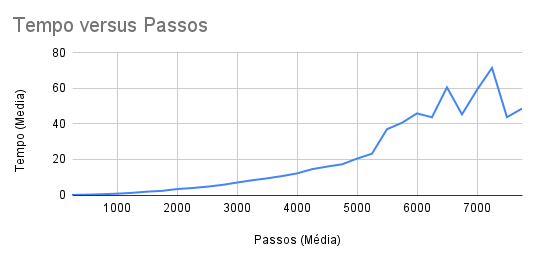
\includegraphics[width=\textwidth]{Imagens/Analises/G_PR2.png}
    \caption{\label{Grafico5} Gráfico da curva de PR como entradas do algoritmo \textit{Greedy}.}
  \end{minipage}
\end{figure}
    
\subsection{Permutações geradas por reversões aleatórias}
    
A figura \ref{Grafico6} mostra o gráfico de nossos testes sobre PGRs como entrada do algoritmo \textit{Greedy}. Os resultados foram calculados a partir da média de 100 testes com permutações de tamanho fixo de 100 elementos, com a a quantidade de reversões de embaralhamento variando de 1 à 200, incrementadas em 5 a cada teste. Verificamos um comportamento através da curva do gráfico que a medida que aumentamos a quantidade de reversões de embaralhamento, a quantidade de reversões para ordenação também cresce. Porém, a partir de um determinado ponto, a curva achata e a média da quantidade de reversões necessárias para ordenação se mantém. Este comportamento se dá pelo fato de que dentro de permutações de tamanho fixo (ou seja, que não variam), não é possível torná-las mais difíceis de se ordenar indeterminadamente apenas embaralhando-as ainda mais. Há um limite para isso e quando esse limite é alcançado, a quantidade de reversões necessárias para se ordenar a permutação torna-se independente da quantidade de reversões de embaralhamento (veja a Propriedade \ref{prop4}). O limite que encontramos neste cenário de testes está entre 70 e 75 reversões de embaralhamento. 

\begin{figure}[H]
  \centering
  \begin{minipage}[t]{0.8\textwidth}
    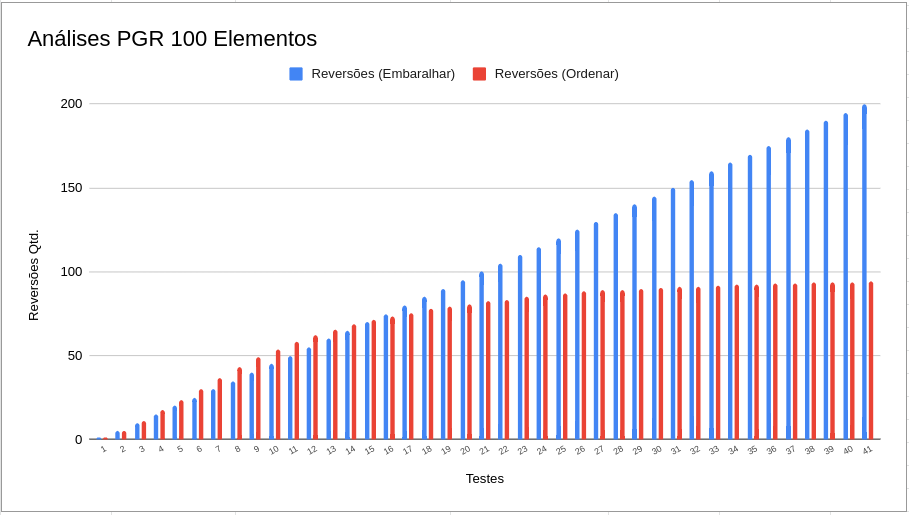
\includegraphics[width=\textwidth]{Imagens/Analises/G_PGR2.png}
    \caption{\label{Grafico6} Gráfico de  barras comparativas de reversões usando PGR como entrada do algoritmo \textit{Greedy}.}
  \end{minipage}
\end{figure}


\section{\textit{Greedy vs.~Branch and Bound}}


Nesta última análise temos um comparativo dos dois algoritmos que implementamos utilizando PGRs como entrada. Utilizamos permutações de tamanho fixo de 30 elementos e variamos a quantidade de reversões de embaralhamento num intervalo de 4 à 16 reversões, com os resultados obtidos a partir de uma média de 20 testes. Na figura \ref{Grafico7} podemos visualizar que ambas as curvas dos algoritmos acompanham o crescimento da curva de embaralhamento. Porém, a curva de crescimento do algoritmo exato (linha amarela) se mantém abaixo da curva de crescimento principal (linha azul), demonstrando que consome em média uma quantidade de passos inferior em relação à quantidade de passos do algoritmo de aproximação, um comportamento que é esperado.

\begin{figure}[H]
  \centering
  \begin{minipage}[t]{0.6\textwidth}
    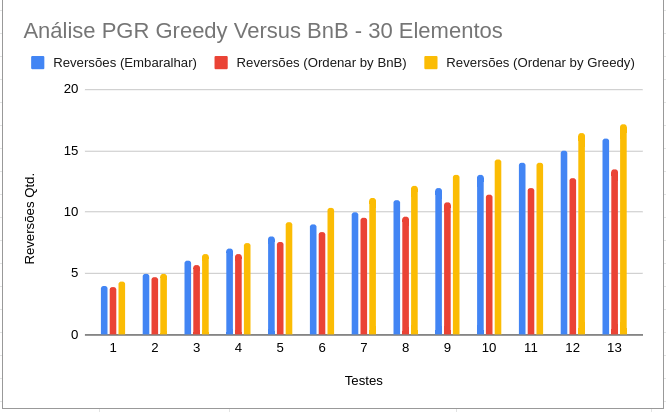
\includegraphics[width=\textwidth]{Imagens/Analises/BG_PGR.png}
    \caption{\label{Grafico7} Gráfico comparativo entre as soluções dos algoritmos \textit{Greedy} e \textit{branch and Bound}.}
  \end{minipage}
\end{figure}
    
Mantivemos um intervalo pequeno na quantidade de reversões, pois dado que o desempenho do algoritmo exato não é bom, há complicações para solucionar instâncias maiores devido ao tempo gasto para ordenar as permutações. Visto isso, descartamos do gráfico informações relativas ao tempo e focamos apenas na quantidade média de reversões necessárias para ordenar as permutações. Pressupomos também que estendendo este experimento teríamos o achatamento das curvas vermelha e amarela, pois como explicado na Propriedade \ref{prop4}, existe um limite do quanto se pode dificultar o processo de ordenação por reversões de uma permutação. 

% \FV{Olhe o rótulo na linha acima (??): lema3 não existe.}

\end{chapter}